%%
%% 2019 07 04 Ph. G. Freimann
%%

\section{Koordinatensystem}\index{Koordinatensystem!kartesisches}\index{Kartesisches
  Koordinatensystem}
\sectuntertitel{Was man nicht gut beschreiben kann, kann man auch
  nicht messen (René Descartes: franz. Philosoph und Mathematiker).}
%%%%%%%%%%%%%%%%%%%%%%%%%%%%%%%%%%%%%%%%%%%%%%%%%%%%%%%%%%%%%%%%%%%%%%%%%%%%%%%%%
\subsection*{Lernziele}

\begin{itemize}
\item $x$-Achse und $y$-Achse\index{Achse}\index{x-Achse}\index{y-Achse}
\item Einheitsstrecke ($e_x$, $e_y$)\index{Einheitsstrecke!im Koordinatensystem}
\item kartesisch (nach René Descartes)\index{kartesisch}
\item Quadrant \index{Quadrant}
\item Ursprung\index{Ursprung}, Nullpunkt
\end{itemize}

\TALS{(\cite{frommenwiler17alg} S. 165 (Kap. 3.1))}
\GESO{(\cite{marthaler17}       S.211 (Kap. 13.1))}

\subsection{Das kartesische Koordinatensystem}
In einem Koordinatensystem kann man Zahlenpaare ($P=(x|y)$) als Punkte
darstellen.

\begin{bemerkung}{}{}
  Auch wenn in einigen Lehrbüchern die Bezeichnung $P(x/y)$ für Punkte gebräuchlich ist (\cite{frommenwiler17alg}), ist
  sie jedoch die unglücklichste von allen. Gerade bei $P=(1/2,5)$
  treten im deutschsprachigen Raum Verwechslungen auf. Ist $P=(1/2,5)$
  nun gleich $P=(1 | 2.5)$ oder gleich $P=(\frac{1}{2} | 5)$?
  Daher verwende ich lieber den senkrechten Strich, was auch in den
  BMS Abschlussprüfungen so gehandhabt wird. Im Lehrbuch wird jedoch
  konsequent der Divisionsstrich ($/$) verwendet, sodass hier auch
  keine Verwechslung auftreten kann.
\end{bemerkung}
\newpage

\subsection{Bezeichnungen im Koordinatensystem}

\TRAINER{\begin{center}\index{Quadrant}\index{$x$-Achse}\index{y-Achse}\index{Ursprung}
  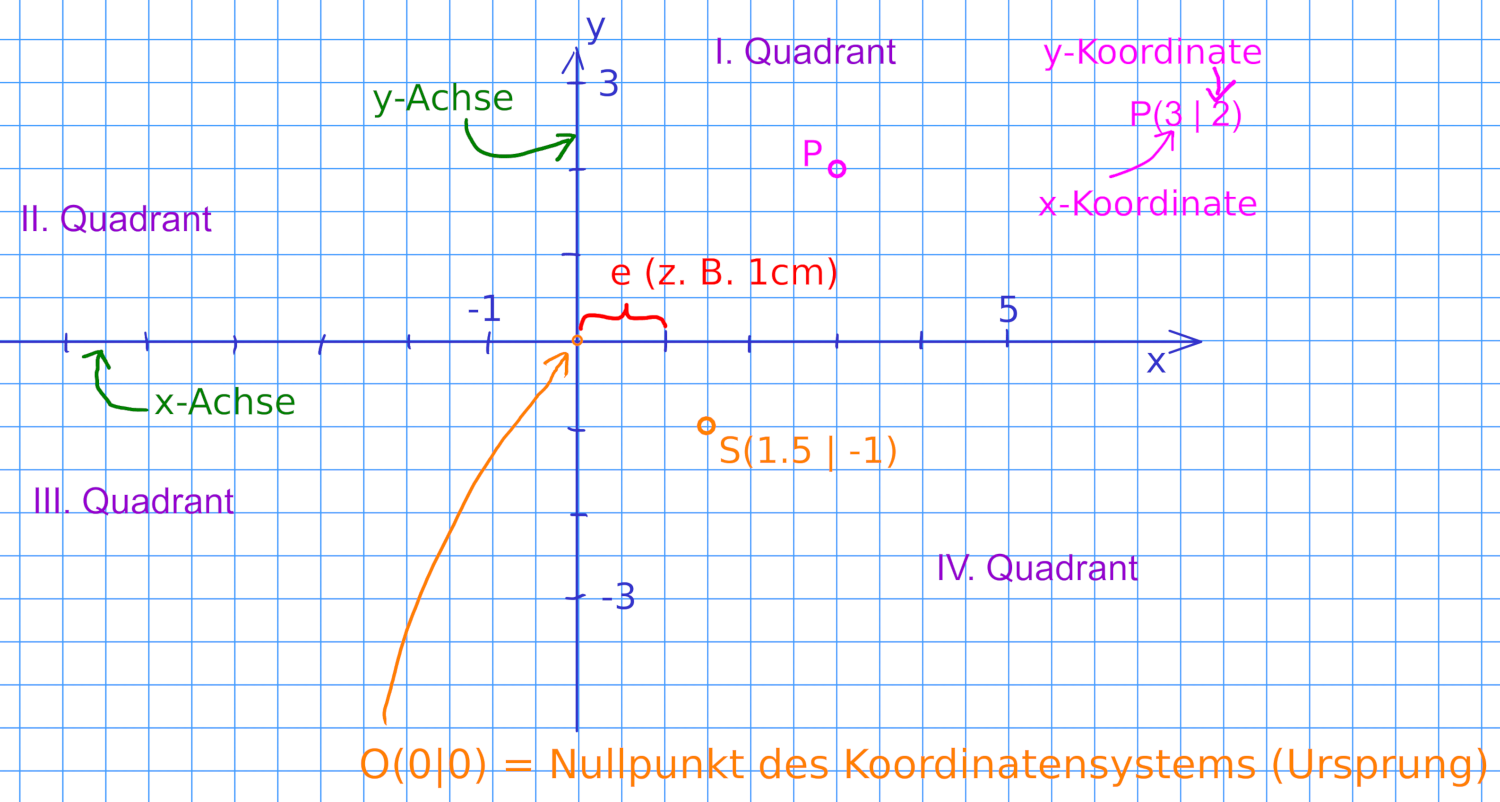
\includegraphics[width=16cm]{allg/funktionen/img/Koordinatensystem.png}
  \end{center}
  \vspace{15mm}
}
\noTRAINER{\bbwGraph{-7}{8}{-4}{5}{}}

\subsection*{Aufgaben}

\TALSAadB{165}{577. e) f) 578. b) 579. a) c) 580. a) c) 581. b) 582.}
\GESOAadB{228ff.}{3. 4. a) b) 5. a) d) e) 7. b) c) 8. a) b) 10. a) c)}
\newpage
